\renewcommand{\arraystretch}{1.5}
\chapter[Präsentatoren\lilib{LILLYxPRESENTER}{1.0.0}]{Präsentatoren}
\TitleSUB{Alles daran setzen, die Dinge hübsch aussehen zu lassen.\hfill \LILLYxBOXxVersion{\small 2.0.0}}
\bigskip\newline
\elable{chp:PRESENTER}\hypertarget{LILLYxPRESENTER}Dieses Paket liegt hier: \begin{center}
    \blankcmd{LILLYxPATHxPRESENTER} = \T{\LILLYxPATHxPRESENTER}
\end{center}
\begin{bemerkung}[Präsentatoren standalone]
    Mit \LILLYxBOXxVersion{2.0.0} wurden die Präsentatoren als eigenes Paket \LILLYxNOTExLibrary{LILLYxPRESENTER} etabliert, welches sich eigenständig über \begin{latex*}
\usepackage{LILLYxPRESENTER}
        \end{latex*}
        auch ohne das Verwenden der restlichen LILLY-Welt benutzen lässt.
\end{bemerkung}

Dem Paket können Argumente übergeben werden, die das Laden einer Bibliothek verhindern, so kann mit \LILLYxBOXxVersion{2.1.0} eingeschränkt werden, welche Pakete geladen werden sollen. \T{iall} lädt alle Argumente:
\begin{center}
    \begin{tabular}{^t^t^>{\raggedright\arraybackslash}p{8cm}+}
        \toprule
            \headerrow Aktivieren & Deaktivieren & Paket \\
        \midrule
            poems & nopoems & \LILLYxNOTExLibrary{LILLYxPOEMS} \\
            ornaments & noornaments & \LILLYxNOTExLibrary{LILLYxORNAMENTS} \\
            tables & notables & \LILLYxNOTExLibrary{LILLYxTABLES}, \LILLYxNOTExLibrary{LILLYxTABLESxMATERIAL}, \LILLYxNOTExLibrary{LILLYxTABLESxFOREACH}  \\
            timetables & notimetables & \LILLYxNOTExLibrary{LILLYxTIMETABLES}, \LILLYxNOTExLibrary{LILLYxTIMETABLESxCOMFORT}, \LILLYxNOTExLibrary{LILLYxTIMETABLESxUNIVERSITY} \\
            persons & nopersons & \LILLYxNOTExLibrary{LILLYxPERSONS}, \LILLYxNOTExLibrary{LILLYxTRANSCRIPTS} \\
            formatcontrol & noformatcontrol & \LILLYxNOTExLibrary{LILLYxFORMATxCONTROL} \\
            utilpresenter & noutilpresenter & \LILLYxNOTExLibrary{LILLYxROTARYxENCODER}, \LILLYxNOTExLibrary{LILLYxSHOWCASE}, \LILLYxNOTExLibrary{LILLYxPROGRESSBARS}\\
            presentgames & nopresentgames & \LILLYxNOTExLibrary{LILLYxCARDS} \\
        \bottomrule
    \end{tabular}
\end{center}
Es gilt zu beachten, dass Abhängigkeiten untereinander dazu führen können, dass Pakete geladen werden, die abgewählt sind. All diese Argumente können auch LILLY übergeben werden um die entsprechenden Module zu konfigurieren. Das Laden des gesamten Pakets \LILLYxNOTExLibrary{LILLYxPRESENTER} kann durch die LILLY-Option \T{nppresenter} verhindert und durch \T{presenter} wieder aktiviert werden.

\section{Generelles}

%
%
%
%
%

\subsection{Formatierungen}
\hypertarget{LILLYxFORMATxCONTROL}Diese Definitionen werden über die Bibliothek \LILLYxNOTExLibrary{LILLYxFORMATxCONTROL} zur Verfügung gestellt. Sie werden mit \LILLYxBOXxVersion{2.0.0} automatisch mit dem Einbinden von \LILLYxNOTExLibrary{LILLYxPRESENTER} geladen.

%
%
%

\presentCommand[2.0.0]{NoFormatChar}
Definiert das Zeichen, welches im Folgenden Befehl verwendet werden kann um eine spezifishe Formtierung zu deaktivieren. Standartmäßig ist dies das Zeichen \T{|} (ein senkrechter Strich/Pipe-Symbol), lässt sich aber jederzeit ändern.

%
%
%

\presentCommand[2.0.0]{lilly@format@iter}[\frmttxt{Value} \blankcmd{@nil}]
Liefert einen normalen Iterator, der über die durch Leerfelder getrennten Tokens eines Satzes iteriert. Für jedes Wort wird \blankcmd{lilly@format@step} mit dem aktuell in \blankcmd{LILLY@FORMATTER@CURRENT} gespeicherten Befehl aufgerufen. Dieser Aufruf separiert das jeweilige Wort mit dem ersten Buchstaben und überprüft die Anwendung des Befehls auf \blankcmd{NoFormatChar}.

%
%
%

\presentCommand[2.0.0]{Acronym}[\manArg{Sentence}]
Formatiert den übergebenen Text so, dass jeder erste Buchstabe eines Wortes fett gedruckt wird. Hierbei wird der Befehl \blankcmd{TextBfFormat} verwendet, der hier nicht dokumentiert ist, weil er an sich nur auf \blankcmd{textbf} verweist und aus Lesbarkeitsgründen umbenannt wurde.
\begin{latex*}
\Acronym{x Wie geht |es ||dir?} % :yields: !*\lstcomment{\Acronym{x Wie geht |es ||dir?}}*!
\end{latex*}
Die Definition von \blankcmd{Acronym} zeigt weiter, wie sich leicht durch die mitgelieferten Befehle ein ähnlicher Befehl definieren lässt:
\begin{latex}[morekeywords={[5]{\\LILLY@FORMATTER@CURRENT,\\lilly@format@iter,\\@Acronym}}]
\def!**!\Acronym!**!#1{% Not Nested
  \gdef!**!\LILLY@FORMATTER@CURRENT{\TextBfFormat}%
  \def!**!\@Acronym{\lilly@format@iter!**!#1 \@nil}{\ignorespaces!**!\@Acronym}%
}
\end{latex}
Allgemein genügt das Abändern von \blankcmd{TextBfFormat} zu einem beliebigen anderen Befehl, der ein Argument akzeptiert. Dieser erhält dann jeweils das erste Zeichen des Wortes und kann es so formatieren wie es gewünscht ist.

%
%
%

\presentCommand[2.0.0]{PoliteWords}[\manArg{Sentence}]
Formatiert den übergebenen Text so, dass jeder erste Buchstabe eines Wortes groß gedruckt wird. Hierbei wird der Befehl \blankcmd{UpperCaseFormat} verwendet, der hier nicht dokumentiert ist, weil er an sich nur auf \blankcmd{MakeUppercase} verweist und aus Lesbarkeitsgründen umbenannt wurde.
\begin{latex*}
\PoliteWords{x Wie geht |es ||dir?} % :yields: !*\lstcomment{\PoliteWords{x Wie geht |es ||dir?}}*!
\end{latex*}

%
%
%

\presentCommand[2.0.0]{ColorfulWords}[\manArg{Sentence}]
Formatiert den übergebenen Text so, dass jeder erste Buchstabe eines Wortes farbig gedruckt wird. Hierbei wird der Befehl \blankcmd{HighlightFormat} verwendet, der hier nicht dokumentiert ist, weil er an sich nur auf \T{\blankcmd{textcolor}\manArg{\blankcmd{Hcolor}}\manArg{\#1}} verweist und aus Lesbarkeitsgründen umbenannt wurde.
\begin{latex*}
\ColorfulWords{x Wie geht |es ||dir?} % :yields: !*\lstcomment{\ColorfulWords{x Wie geht |es ||dir?}}*!
\end{latex*}

%
%
%

\presentCommand[2.0.0]{doublealph}[\manArg{counter}]
Während das durch \LaTeX\ definierte \blankcmd{alph} nur für Werte $1$--$26$ definierte ist, definiert dieser Befehl die \blankcmd{ifcase}-Anweisung für die Werte $1$--$702$:
\bgroup\newcounter{einzähler}%
\begin{latex}
\newcounter{einzähler}
\setcounter{einzähler}{1}
\doublealph{einzähler}      % :yields: !*\lstcomment{\setcounter{einzähler}{1}\doublealph{einzähler}}*!
\setcounter{einzähler}{42}
\doublealph{einzähler}      % :yields: !*\lstcomment{\setcounter{einzähler}{42}\doublealph{einzähler}}*!
\setcounter{einzähler}{702}
\doublealph{einzähler}      % :yields: !*\lstcomment{\setcounter{einzähler}{702}\doublealph{einzähler}}*!
\doublealph{section}        % :yields: !*\lstcomment{\doublealph{section}}*!
\doublealph{page}           % :yields: !*\lstcomment{\doublealph{page}}*!
\end{latex}
\egroup

%
%
%
%
%

\subsection{Ornamente}
\hypertarget{LILLYxORNAMENTS}Diese Definitionen werden über die Bibliothek \LILLYxNOTExLibrary{LILLYxORNAMENTS} zur Verfügung gestellt. Sie werden mit \LILLYxBOXxVersion{2.0.0} automatisch mit dem Einbinden von \LILLYxNOTExLibrary{LILLYxPRESENTER} geladen.\medskip\newline
Das folgende Paket definiert eine unglaubliche Anzahl an Befehlen, die nicht alle im Index aufgeführt werden.

%
%
%

\presentCommand[2.0.0]{@@CreateOrnamentCommand}[\manArg{Number}\manArg{Name}\manArg{Defaultargs}]
Konstruiert einen Neuen Befehl der Struktur \blankcmd{orna<Name>}, der auf das \blankcmd{pgfornament} mit der entsprechenden \T{Number} abbildet. Weiter werden die \T{Defaultargs} übergeben, die ab da bei jedem Aufruf des Befehls Standartmäßig übergeben werden. Weiter registriert sich das Ornament in der durch \LILLYxNOTExLibrary{LILLYxLIST} bereitgestellten Liste \T{RegisteredOrnaments}

%
%
%

\presentCommand[2.0.0]{orna<Name>}[\optArg{ornaargs}]
Setzt das zuvor mit \blankcmd{@@CreateOrnamentCommand} definierte Ornament. So zum Beispiel: \blankcmd{ornalion} liefert \ornalion.
Hier eine Auflistung aller Ornamente:
\getRegisteredOrnaments%
%\edef\xdoctmp{\noexpand\typesetList{\lillyxlist}}\xdoctmp
\expandafter\typesetList[T]{\lillyxlist}

%
%
%

\presentCommand[2.0.0]{OrnamentsBoxTitle}[\optArg{tikzargs}\manArg{Title}\optArg{width}]
Setzt eine Ornamentbox um den \T{Title}, wobei die Breite automatisch auf Basis der Länge des Titels generiert wird, sofern sie nicht durch \T{width} explizit angegeben wird.
\iflillycompact%
\begin{latex}
    \begin{center}
        \OrnamentsBoxTitle{Hallo}
    \end{center}
\end{latex}
\else%
\begin{defaultlst}[][listing side text,righthand width=7cm]{lLatex}
\begin{center}
    \OrnamentsBoxTitle{Hallo}
\end{center}
\end{defaultlst}
\fi%

%
%
%

\presentCommand[2.0.0]{OrnamentsUpper}[\optArg{Ornament Right}\optArg[ornafeather]{Ornament Left}\secline\optArg{tikz args}\manArg{Title}\cmdlist\anothercmd[2.0.0]{OrnamentsLower}\optArg{tikz args}\manArg{TextRight}]
Setzt obere und untere Begrenzer, die auch in \LILLYxNOTExLibrary{LILLYxPOEMS} verwendet werden.
\begin{defaultlst}{lLatex}
\OrnamentsUpper{Meldung}

\OrnamentsLower{Wichtig!}
\end{defaultlst}
\iflillycompact\else Ergibt:\\
\OrnamentsUpper{Meldung}

\OrnamentsLower{Wichtig!}\fi
Information: Die Breite dieser Begrenzer passt sich an die aktuelle Zeilenbreite an, ist allerdings(bezüglich Liniendicke) auf Seiten im \T{DIN A4}-Format optimiert.

%
%
%

\presentCommand[2.0.0]{PresentAllOrnaments}
Erzeugt mithilfe von \LILLYxNOTExLibrary{LILLYxTABLESxFOREACH} eine tabellarische Auflistung aller Ornamente.
\begin{example}
    \begin{tcbraster}[raster columns=4, blankest, graphics pages={1,2,6}, colback=white]
        \tcbincludepdf{Data/Documents/AllOrnaments/ornaments.pdf}
    \end{tcbraster}
\end{example}
Die unterschiedlichen Höhen entstammen hierbei der Tatsache, dass dieser Befehl alle Ornamente (zur besseren Übersicht) mit derselben Breite setzt.

%
%
%
%
%

\subsection{Fortschrittsanzeigen}
\hypertarget{LILLYxPROGRESSBARS}Diese Definitionen werden über die Bibliothek \LILLYxNOTExLibrary{LILLYxPROGRESSBARS} zur Verfügung gestellt. Sie werden mit \LILLYxBOXxVersion{2.1.0} automatisch mit dem Einbinden von \LILLYxNOTExLibrary{LILLYxPRESENTER} geladen.

%
%
%

\presentCommand[2.1.0]{ProgressBar}[\optStar\optArg{tikz}\manArg{drawer}\manArg{progress}\optArg[\blankcmdidx{Hcolor}]{border}\secline\optArg[\blankcmdidx{Hcolor}]{progres}\optArg{background}\optArg[6.5em]{width}\optArg[MudWhite]{text}]
Zeichnet eine Fortschrittsanzeige im Stil \T{drawer} mit einem Fortschritt von \T{progress}\%. Wird der Stern gesetzt, so wird versucht den prozentualen Fortschritt anzuzeigen, die Option wurde eigentlich nur für einen \T{drawer} konzipiert und ist deswegen unter Umständen sinnfrei. Es werden die folgenden \T{drawer} unterstützt: \typesetList[T]{roundings,rounds,triangles,hexas,slider,dots,radial,radialbars,radialdots}. Der Fortschritt kann auch als Zahl $p \in [0,1]$ angegeben werden. Hier ein paar Beispiele:
\begin{defaultlst}[][listing side text,righthand width=3.5cm]{lLatex}
\ProgressBar{roundings}{27}
\ProgressBar{rounds}{100}
\ProgressBar{triangles}{0.13}
\ProgressBar{hexas}{85}
\ProgressBar{slider}{55}
\end{defaultlst}
Die mit \T{radial} angeführten Fotschrittsleisten benötigen entsprechend mehr Platz und lassen sich somit auch nicht in einen normalen Textfluss einbinden:
\iflillycompact
\begin{latex}
\ProgressBar{radialbars}{27}
\ProgressBar{radial}{45}
\ProgressBar{radialdots}{0.9251}
\end{latex}
\else
\begin{defaultlst}[][listing above text,righthand width=3.5cm,before lower={\centering}]{lLatex}
\ProgressBar{radialbars}{27}
\ProgressBar{radial}{45}
\ProgressBar{radialdots}{0.9251}
\end{defaultlst}
\fi
%
%
%
%
%

\section{Tabellen}
\hypertarget{LILLYxTABLES}Diese Definitionen werden über die Bibliothek \LILLYxNOTExLibrary{LILLYxTABLES} zur Verfügung gestellt. Sie werden mit \LILLYxBOXxVersion{2.0.0} automatisch mit dem Einbinden von \LILLYxNOTExLibrary{LILLYxPRESENTER} geladen.\medskip\newline

In diesem Paket werden einige neue Spaltentypen definiert, die Problemlos in so ziemlich jeder Tabelle verwendet werden können:
\begingroup\footnotesize
\begin{multicols}{2}
    \begin{description}
        \foreach \c/\brief in {%
            b/Fettgedruckt (l),%
            u/Mathematisch (c),%
            g/Fußnotengröße (l),%
            w/Fußnotengröße (X),%
            i/Kursiv (l),%
            L\{\#\}/linskbündige m-Spalte der Breite \#,%
            R\{\#\}/rechtsbündige m-Spalte der Breite \#,%
            C\{\#\}/zentrierte m-Spalte der Breite \#,%
            t/Spalte mit \blankcmd{LILLYxlstTypeWriter} (l),%
            T\{\#\}/linksbündige p-Spalte der Breite \# in \blankcmd{LILLYxlstTypeWriter}-Schrift,%
            \_/Abstand von $3em$,%
            \textasciitilde/Abstand von $1.5em$,%
            ./Spaltenabstand von $1.5em$%
        }{%
            \item[\c] \brief
        }
    \end{description}
\end{multicols}
\endgroup

%
%
%

\presentCommand[2.0.0]{setrow}[\manArg{Commands}]
Setzt Befehle, die in dieser Zeile jeder Zelle vorangesetzt werden soll. Dieser Befehl lässt sich allerdings nicht einfach so verwenden, da ein derartiges Verhalten in Umgebungen wie \blankenv{tabular} nicht vorgesehen ist. Jede Spalte auf die ein derartiger Effekt angewendet werden soll muss in der Definition mit einem \T{\^{}} angeführt, die Spaltendefinition an sich wiederrum mit einem \T{+} abgeschlossen werden. Im Folgenden ein Beispiel:
\begin{defaultlst}[][listing side text,righthand width=3.5cm]{lLatex}
\begin{tabular}{^l^c^r+}
    Wir & sind & normal \\
    \setrow{\itshape} Wir & sind & kursiv \\
    Wir & sind & normal \\
    \setrow{\bfseries} Wir & sind & fett
\end{tabular}
\end{defaultlst}

%
%
%

\presentCommand[2.0.0]{clearrow}
Löscht den durch \blankcmd{setrow} erzeugten Zeilenmodifikator:
\begin{defaultlst}[][listing side text,righthand width=3.5cm]{lLatex}
\begin{tabular}{^l^c^r+}
    Wir & sind & normal \\
    \setrow{\itshape} Wir & sind & kursiv \\
    Wir & sind & normal \\
    \setrow{\bfseries} Wir & sind \clearrow& fett
\end{tabular}
\end{defaultlst}
Dies wird durch \T{+} automatisch am Ende der Zeile angefügt.

%
%
%

\presentCommand[2.0.0]{headerrow}[\optStar]
Setzt mithilfe von \blankcmd{setrow} eine Kopfzeile, der Stern behält die Grundlegende Formatierung der jeweiligen Zeile bei, sonst werden etwaige Formatierungen entfernt:
\begin{defaultlst}[][listing side text,righthand width=3.5cm]{lLatex}
\begin{tabular}{^i^t^r+}
    \headerrow  Wir   & sind  & normal \\
    \headerrow* Eine  & tolle & Zeile \\
                Super & tolle & Zeile
\end{tabular}
\end{defaultlst}

%
%
%

\presentCommand[2.0.0]{cheaderrow}[\cmdlist\anothercmd[2.0.0]{normalrow}\cmdlist\anothercmd[2.0.0]{smallrow}\cmdlist\anothercmd[2.0.0]{footnotesizerow}\cmdlist\anothercmd[2.0.0]{scriptsizerow}\cmdlist\secline\anothercmd[2.0.0]{tinyrow}]
Setzt mithilfe von \blankcmd{setrow} entsprechend formatierte Zeilen:
\begin{defaultlst}[][listing side text,righthand width=3.5cm]{lLatex}
\begin{tabular}{^i^c^r+}
    \cheaderrow  Eine & tolle & Zeile \\
    \normalrow   Eine & tolle & Zeile \\
    \smallrow    Eine & tolle & Zeile \\
    \footnotesizerow    Eine  & tolle & Zeile \\
    \scriptsizerow      Eine  & tolle & Zeile \\
    \tinyrow     Eine & tolle & Zeile
\end{tabular}
\end{defaultlst}

%
%
%
%
%

\subsection{Iterationen}
\hypertarget{LILLYxTABLESxFOREACH}Diese Definitionen werden über die Bibliothek \LILLYxNOTExLibrary{LILLYxTABLESxFOREACH} zur Verfügung gestellt. Sie werden mit \LILLYxBOXxVersion{2.0.0} automatisch mit dem Einbinden von \LILLYxNOTExLibrary{LILLYxPRESENTER} geladen.

%
%
%

\presentCommand[2.0.0]{tabadd}[\manArg{tokens}\cmdlist\anothercmd[2.0.0]{etabadd}\manArg{tokens}]
Fügt die \T{tokens} dem aktuellen Speicher (\blankcmd{@@tabular@tokens}) hinzu. Zu beachten ist, dass \blankcmd{etabadd} die \T{Tokens} mittels \blankcmd{edef} expandiert.

%
%
%

\presentCommand[2.0.0]{tabreset}
Leert den durch \blankcmd{tabadd}/\blankcmd{etabadd} erzeugten Speicher. Sollte, um sicher zu gehen, vor jeder neuen Iteration getätigt werden.

%
%
%

\presentCommand[2.0.0]{tabprint}
Gibt die aktuellen Tokens aus. Hier ein Beispiel:
\begin{defaultlst}[][listing side text,righthand width=3.5cm]{lLatex}
\tabreset%
\foreach \i in {1,...,5} {%
    \etabadd{Zeile \i}%
    \tabadd{ & Hallo Welt \\}%
}%
\begin{tabular}{ll}
    \tabprint
\end{tabular}
\end{defaultlst}

%
%
%

\presentCommand[2.0.0]{tabforeach}[\manArg{Var}\manArg{Elements}\manArg{Body}]
Vereinfachte Möglichkeit um eine Tabelle so zu generieren.
\begin{defaultlst}[morekeywords={[5]{\\amp}}][listing side text,righthand width=3.5cm]{lLatex}
\tabforeach{\i}{1,...,5}{%
    \etabadd{Zeile \i \amp Hallo Welt}
}
\begin{tabular}{ll}
    \tabprint
\end{tabular}
\end{defaultlst}
Der Befehl \blankcmd{amp} steht nur innerhalb von \blankcmd{tabforeach} zur Verfügung und erlaubt so das setzen von einem \T{\&} innerhalb von \blankcmd{etabadd}, was es hier ermöglicht den weiteren Aufruf zu \blankcmd{tabadd} einspahrt. Das Zeilenende wird automatisch am Ende jeder Iteration angefügt, \blankcmd{tabreset} wird automatisch aufgerufen.

%
%
%
%
%
\clearpage % For Pagebreak @ mltable:D
\subsection{Weitere Designs}
\hypertarget{LILLYxTABLESxMATERIAL}Diese Definitionen werden über die Bibliothek \LILLYxNOTExLibrary{LILLYxTABLESxMATERIAL} zur Verfügung gestellt. Sie werden mit \LILLYxBOXxVersion{2.0.0} automatisch mit dem Einbinden von \LILLYxNOTExLibrary{LILLYxPRESENTER} geladen.

\begin{bemerkung}[Das tabu-Paket und seine Leiden]
    Die Bibliothek \LILLYxNOTExLibrary{LILLYxTABLESxMATERIAL} wurde erst auf Basis des tabu-Pakets (\url{https://www.ctan.org/pkg/tabu}), da das Paket seit $2011$ nichtmehr aktiv entwickelt wird unktuell ohne Maintainer vor sich hin vegetiert, ist es möglich, dass die durch Lilly etablierten Fixes und Variationen dennoch nicht funktionieren, was manche der folgenden Tabellen nicht \say{gut} aussehen lässt oder sogar unbrauchbar macht.
\end{bemerkung}

%
%
%

\presentEnvironment[2.0.0]{mtable}[\optStar\optArg[\blankcmdidx{MHeaderRow}]{Headerrow}\optArg{PreCode}\manArg{Header}\secline\optArg[MudWhite!10]{FirstRow}\optArg[MudWhite!90]{Second Row}]
Setzt eine Tabelle in einem an das Material-Design des Editor Atom angelehnten Design:
\begin{defaultlst}[][listing side text,righthand width=3.5cm]{lLatex}
\begin{mtable}{ll}
    Hallo & Welt \\
    Na & Wie \\
    geht & es \\
    dir & denn?
\end{mtable}
\end{defaultlst}
Die Variante mit einem Stern, besitzt keine explizite Formatierung der Kopfzeile.

\presentEnvironment[2.0.0]{mltable}[\optStar\optArg[\blankcmdidx{MHeaderRow}]{Headerrow}\optArg{PreCode}\manArg{Header}\secline\optArg{Mulitpage Header}\optArg[MudWhite!10]{FirstRow}\secline\optArg[MudWhite!90]{Second Row}\optArg[\blankcmdidx{MNHeaderRow}]{Next Headerrow}]
Setzt eine Tabelle, die gut und gerne über mehere Seiten gehen kann. Die Kopf-Zeile(n) die auf allen Seiten oben stehen soll(en), werden nach den Spaltendefinitionen als optionales Argument angenommen:
\begin{mltable}{llr}[Spalte 1 & Super & Hey]
    Hallo & Welt & Na \\
    Wie & geht & es \\
    dir & denn? & Ich \\
    mag & Züge & ! \\
    Und & Ich & bin \\
    eine & echt & lange \\
    Tabelle & findest & du \\
    nicht & auch & ? \\
    Shubi & dubi & duuu \\
    Das ist doch & Wirklich super & tolle dolle \\
    Mir fehlen & die Worte & Ich horte \\
    Die Tabelle & sehr lange & oh bange!
\end{mltable}

Ich habe den Code hier einmal separiert, um auch wirklich einen Zeilenumbruch an der Stelle zu forcieren können:

\begin{latex}
\begin{mltable}{llr}[Spalte 1 & Super & Hey]
    Hallo & Welt & Na \\
    Wie & geht & es \\
    dir & denn? & Ich \\
    mag & Züge & ! \\
    Und & Ich & bin \\
    eine & echt & lange \\
    Tabelle & findest & du \\
    nicht & auch & ?
\end{mltable}
\end{latex}
Der zugehörige kleine Pfeil in den fortgeführten Kopfzeilen definiert der Befehl \blankcmd{MNHeaderRow}. In der Regel sollte man annehmen, dass die Verwendung von \blankenv{mltable} einen zweiten Kompiliervorgang erfordert.

%
%
%

\presentCommand[2.0.0]{MHeaderRow}[\cmdlist\anothercmd[2.0.0]{MNHeaderRow}]
Definieren die Gestalt der Kopfzeilen, wobei \blankcmd{MNHeaderRow} speziell nach Seitenumbrüchen angewandt wird. Hier gilt zu beachten, dass die Umgebungen \blankenv{mtable} und \blankenv{mltable} diese nur als Standardeinstellung nutzen und somit auch die Verwendung der Befehle für einzelne Argumente ausgeschaltet werden kann. Standardmäßig unterscheiden sich die beiden Befehle übrigens nur in der Hinsicht, dass \blankcmd{MNHeaderRow} noch ein kleines Dreieck an die linke Tabellenseite setzt. Sie verwenden die Farben \emph{HeaderColor} sowie \emph{NextHeaderColor}, die initial beide auf \blankcmd{Hcolor} gesetzt werden, aber jederzeit überschreibbar sind. \medskip

\begin{bemerkung}[Der versuchte Ersatz \Smiley]
    Um den Problemen von \T{tabu} entgegenzuwirken liefert \LILLYxNOTExLibrary{LILLYxTABLESxMATERIAL} noch zwei provisorische Umgebungen. Diese verwenden \blankcmd{@@tabularArgPatch@iter}, welches automatisch die für \blankcmd{setrow} benötigten Konfigurationen \T{\^{}} und \T{+} einfügt (allerdings auch vor Befehlen und anderen Zeichen was bedeutet, dass wirklich nur Spalten akzeptiert werden. Dies hat den Nachteil, dass neue Spalten erstellt werden müssen, wenn verschiedene Befehle gewünscht sind!).
\end{bemerkung}

%
%
%

\presentEnvironment[2.0.0]{mtabular}[\optStar\optArg[\blankcmdidx{MTBHeaderRow}]{Headerrow}\optArg{PreCode}\manArg{Header}\secline\optArg[MudWhite!10]{FirstRow}\optArg[MudWhite!90]{Second Row}]
Setzt eine Tabelle in einem an das Material-Design des Editor Atom angelehnten Design:
\begin{defaultlst}[][listing side text,righthand width=3.5cm]{lLatex}
\begin{mtabular}{ll}
    Hallo & Welt \\
    Na & Wie \\
    geht & es \\
    dir & denn?
\end{mtabular}
\end{defaultlst}
Die Variante mit einem Stern, besitzt keine explizite Formatierung der Kopfzeile.
Es gilt zu beachten, das Lilly für diese Tabellen eine eigene Version des Pakets \T{xcolor} (\url{https://www.ctan.org/pkg/xcolor}) mitführt, um auch ältere Latex-Versionen zu unterstützen! Sollte dieses Verhalten zu Problemen führen, so kann dies durch die Definition von \blankcmd{LILLYxUSEREGXCOLOR} vor dem Einbinden von Lilly deaktiviert werden!


%
%
%

\presentEnvironment[2.0.0]{mltabular}[\optStar\optArg[\blankcmdidx{MTBHeaderRow}]{Headerrow}\optArg{PreCode}\manArg{Header}\secline\optArg{Mulitpage Header}\optArg[MudWhite!10]{FirstRow}\secline\optArg[MudWhite!90]{Second Row}\optArg[\blankcmdidx{MNTBHeaderRow}]{Next Headerrow}]
Setzt eine Tabelle in einem an das Material-Design des Editor Atom angelehnten Design:
\begin{mltable}{llr}[Spalte 1 & Super & Hey]
    Hallo & Welt & Na \\
    Wie & geht & es \\
    dir & denn? & Ich
    % ...
\end{mltable}
Und hier der Code:
\begin{latex}
\begin{mltable}{llr}[Spalte 1 & Super & Hey]
    Hallo & Welt & Na \\
    Wie & geht & es \\
    dir & denn? & Ich
    % ...
\end{mltable}
\end{latex}
Für die Realisierung wird \T{longtable} verwendet!

%
%
%

\presentCommand[2.0.0]{MTBHeaderRow}[\cmdlist\anothercmd[2.0.0]{MNTBHeaderRow}]
Diese Befehle funktionieren analog zu \blankcmd{MHeaderRow} und \blankcmd{MNHeaderRow}, wobei sie die Befehle so abändern, dass sie in den Kompatibiltitätsumgebungen \blankenv{mtabular} und \blankenv{mltabular} funktionieren!

%
%
%
%
%

\section{Gedichte}
\hypertarget{LILLYxPOEMS}Diese Definitionen werden über die Bibliothek \LILLYxNOTExLibrary{LILLYxPOEMS} zur Verfügung gestellt. Sie werden mit \LILLYxBOXxVersion{2.0.0} automatisch mit dem Einbinden von \LILLYxNOTExLibrary{LILLYxPRESENTER} geladen. Dieses Modul macht von \LILLYxNOTExLibrary{LILLYxORNAMENTS} gebrauch!

%
%
%

\presentCommand[2.0.0]{poemssetauthor}[\manArg{Author}]
Setzt den Autor, der standardmäig auf \blankcmd{AUTHOR} gesetzt ist und so als Standardautor für alle folgenden Gedichte verwendet wird.

%
%
%

\presentEnvironment[2.0.0]{poem}[\optArg{Comment}\optArg{Left Ornament}\optArg{Right Ornament}\secline\manArg{Name}\manArg{Date}\optArg[\blankcmdidx{poems@author}]{Author}]
Setzt ein Gedicht mit dem Namen \T{Name} geschrieben am \T{Date}. Der Autor kann durch \blankcmd{poemssetauthor} geändert, oder gezielt durch \T{Author} angegeben werden. Diese umgebung unterscheidet sich von \blankenv{poems*}, dass sie noch einen Seitenumbruch einfügt und das Gedicht auch vertikal zentriert. Allein deswegen wird zum Beibehalt der Dokumentationskonsistenz dort ein entsprechendes Beispiel gezeigt, da sich die Umgebungen sonst gleichen.

%
%
%

\presentEnvironment[2.0.0]{poem*}[\optArg{Comment}\optArg{Left Ornament}\optArg{Right Ornament}\secline\manArg{Name}\manArg{Date}\optArg[\blankcmdidx{poems@author}]{Author}]
Für eine genaue Erklärung siehe \blankenv{poem}. Hier ein Beispiel:
\begin{latex}
\begin{poem*}{Hallo Welt}{10.09.2019}[Florian Sihler]
    Hallo Welt,
    Wie geht es dir?
    Du bist so fern,
    und doch bei mir.
    ich hab dich gern,
    und bin doch hier.
\end{poem*}
\end{latex}
\iflillycompact\else%
    \begin{poem*}{Hallo Welt}{10.09.2019}[Florian Sihler]
        Hallo Welt,
        Wie geht es dir?
        Du bist so fern,
        und doch bei mir.
        ich hab dich gern,
        und bin doch hier.
    \end{poem*}
\fi

\presentCommand[2.0.0]{subduelines}
Wie am Beispiel für \blankenv{poem*} zu sehen ist, müssen keine Zeilenenden oder ähnliches angegeben werden. Dies mag die Verwendung von \blankcmd{obeylines} vermuten lassen, allerdings hätte dieser Befehl den Nachteil, dass die Strophen nicht durch eine Leerzeile getrennt werden könnten, da diese von \blankcmd{obeylines} geschluckt werden. Deswegen stellt dieser Befehl eine Variante dar, die sowohl in zentrierten als auch nicht zentrierten Umgebungen funktioniert:
%Make this preview Latex command :D
\begin{defaultlst}[][listing side text,righthand width=3.5cm]{lLatex}
Mit \blankcmd{subduelines}:
{
    \subduelines
    Hallo Welt,

    Na wie,
    geht

    es dir?
}

\textbf{Zum Vergleich: }\\
Mit \blankcmd{obeylines}:

{
    \obeylines
    Hallo Welt,

    Na wie,
    geht

    es dir?
}
\end{defaultlst}

%
%
%

\presentEnvironment[2.0.0]{quotes}[\optArg[Quotes]{Title}\optArg[\blankcmdidx{poems@author}]{Author}]
Läutet eine Umgebung ein, in der verschiedene, durch \blankcmd{singlequote} oder \blankenv{quote} eingeläutete Zitate definiert werden können. Im Gegensatz zu \blankenv{quotes*}, setzt \blankenv{quotes} einen Rahmen umd die Zitate:
\begin{latex}
\begin{quotes}
    \begin{quote}
        Ein Dieter kommt selten zu zweit.
    \end{quote}
    \begin{quote}[14.42.2422]
        Niemand hat die Absicht die Erde zu sprengen!
    \end{quote}
\end{quotes}
\end{latex}
Ergibt (der Seitenumbruch wird erzwungen \Smiley):
\begin{quotes}[Testzitate]
    \begin{quote}
        Ein Dieter kommt selten zu zweit.
    \end{quote}
    \begin{quote}[14.42.2422]
        Niemand hat die Absicht die Erde zu sprengen!
    \end{quote}
\end{quotes}

%
%
%

\presentEnvironment[2.0.0]{quotes*}[\optArg[\blankcmdidx{poems@author}]{Author}]
Definiert eine Umgebung in der der Befehl \blankcmd{singlequote} und die Umgebung \blankenv{quote}. Diese Umgebung wird von \blankenv{quotes} intern verwendet.

\begin{defaultlst}[][listing side text,righthand width=3.5cm]{lLatex}
\begin{quotes*}
    \singlequote{Hallo}
    \singlequote{Welt}
\end{quotes*}
\end{defaultlst}

%
%
%

\presentCommand[2.0.0]{singlequote}[\manArg{quote}]
Setzt innerhalb einer \blankenv{quotes*}-Umgebung ein einzelnes Zitat, ohne gesonderte Autor oder Datumsangabe, so können mehrere Zitate mit gleichen Metadaten hübsch gesetzt werden:

%
%
%

\presentEnvironment[2.0.0]{quote}[\optArg{Date}]
Setzt unter der Verwendung von \blankcmd{singlequote} ein Zitat mit Autor und optionales Datumsangabe.
\elable{mrk:hidu}
\begin{bemerkung}[Auflistung der Gedichte und Zitate]
    Alle Gedichte können mit \blankcmd{listofPOEMS}, alle Zitate mit \blankcmd{listofQUOTES} gelistet werden. Es kann mithilfe der folgenden Bedinungen abgefragt werden, ob überhaupt ein Gedicht/Zitat im Dokument aufgetaucht ist, so kann \say{verhindert} werden, dass eine leere Liste angezeigt wird (beachte \blankcmd{makeatletter}): \blankcmd{iflist@poems@seen} und \blankcmd{iflist@quotes@seen}. Dieses Verfahren basiert auf \LILLYxNOTExLibrary{LILLYxRECORDER} und verwendet das Suffix \T{POEMSWATCHER}.
\end{bemerkung}

%
%
%
%
%

\section{Stundenpläne}
\hypertarget{LILLYxTIMETABLES}Diese Definitionen werden über die Bibliothek \LILLYxNOTExLibrary{LILLYxTIMETABLES} zur Verfügung gestellt. Sie werden mit \LILLYxBOXxVersion{2.0.0} automatisch mit dem Einbinden von \LILLYxNOTExLibrary{LILLYxPRESENTER} geladen.

%
%
%

\presentCommand[2.0.0]{NewTimeTable}[\optArg{tt keys}\manArg{Name}]
Erzeugt einen neuen Stundenplan, dessen Werte mittels \blankcmd{xdef} persistiert werden (Präfix: \T{lillyxTIMETABLESx}). Neben dem Zähler \T{@<Name>@maxcount} werden die beiden Befehle \blankcmd{the<Name>} und \blankcmd{present<Name>} erzeugt.

Es gibt eine ganze Reihe möglicher \T{tt keys} die übergeben werden können und das endgültige Aussehen des Stundenplans konfigurieren.
\begin{center}
    \begin{tabularx}{\linewidth}{^t>{\em}^l^c^p{0.35\linewidth}+}
        \toprule
            \headerrow Bezeichner & \normalfont\bfseries Typ & Standard & Beschreibung\\
        \midrule
        title & String & \T{Ich bin ein\ldots} & Titel des Stundenplans \\
        bordercolor & Farbe & black & Rahmenfarbe \\
        day start time & Zahl (0-23) & 8 & Tagesstartzeit \\
        day end time & Zahl (0-23) & 20 & Tagesendzeit \\
        week start day & Zahl (0-6) & 0 & Starttag (Montag)\\
        week end day & Zahl (0-6) & 4 & Endtag (Freitag)\\
        time formatter & enum (siehe unten) & AtLineDistCompanion & Formatierung der Zeit \\
        \bottomrule
    \end{tabularx}\nskip
\end{center}
Der \T{time formatter} ist in sofern besonders, dass er zwei Makros fordert, die der Syntax \T{@@TimeFormatter@<Bezeichner>} und \T{@@TimeFormatter@<Bezeichner>@Sequence} folgen und so definieren wie die Zeiten am linken Rand formatiert werden sollen. Die folgenden Werte sind bereits vordefiniert: \typesetList[T]{Default,RevertDefault,AtLine,AtLineCompanion,AtLineDistCompanion}.
Betrachten wir einmal ein Beispiel:
\begin{latex}[morekeywords={[5]{\\theTimeTable}}]
\NewTimeTable[%
    title = Hallo Welt,
    day start time = 12, % Start 12 uhr
    day end time = 16,   % Ende 16 uhr
    week start day = 5,  % Samstag und
    week end day = 6,    % Sonntag
    time formatter = Default
]{TimeTable}
\begin{center}
    \theTimeTable
\end{center}
\end{latex}
\bgroup%
\NewTimeTable[%
    title = Hallo Welt,
    day start time = 12, % Start 12 uhr
    day end time = 16,   % Ende 16 uhr
    week start day = 5,  % Samstag und
    week end day = 6,    % Sonntag
    time formatter = Default
]{TimeTable}
\begin{center}
    \theTimeTable
\end{center}
\egroup%
Ein weiteres Beispiel:
\begin{latex}[morekeywords={[5]{\\theAnotherTimeTable}}]
\NewTimeTable{AnotherTimeTable}
\begin{center}
    \theAnotherTimeTable
\end{center}
\end{latex}
\NewTimeTable{AnotherTimeTable}
\begin{center}
    \theAnotherTimeTable
\end{center}

%
%
%

\presentCommand[2.0.0]{the<Name>}[\cmdlist\anothercmd[2.0.0]{present<Name>}]
Rufen jeweils \blankcmd{DrawTimeTable} beziehungsweise \blankcmd{PresentTimeTable} mit dem entsprechenden Namen als Argument auf.

%
%
%

\presentCommand[2.0.0]{DrawTimeTable}[\manArg{TimeTable}]
Zeichnet den entsprechenden Stundenplan innerhalb einer \blankenv{tikzpicture}-Umgebung.

%
%
%

\presentCommand[2.0.0]{PresentTimeTable}[\manArg{TimeTable}]
Setzt den Stundenplan auf eine neue Seite und setzt die Abstände entsprechend. Intern wird auf \blankcmd{DrawTimeTable} zurückgegriffen.

%
%
%

\presentCommand[2.0.0]{RawTimeTableEvent}[\optArg{tt event keys}\manArg{TimeTable}]
Generiert ein Event im Timetable, wobei automatisch zwei verschiedene Stile je nach Länge des Events angewedet werden.
\begin{center}
    \begin{tabularx}{\linewidth}{^t>{\em}^l^c^p{0.35\linewidth}+}
        \toprule
            \headerrow Bezeichner & \normalfont\bfseries Typ & Standard & Beschreibung\\
        \midrule
        title & String & bummelbahn & Titel des Events \\
        short title & String & & Kurzer Titel des Events \\
        bgcolor & Farbe & AppleGreen!15 & Rahmenfarbe \\
        day & Zahl (0-6) & 0 & Tag des Events \\
        y & Zahl & -1.125 & Vertikale Position des Events \\
        height & Zahl & 1.25 & Länge des Events \\
        preCode & Code & & Code vor dem Event \\
        postCode & Code & & Code nach dem Event \\
        extra 1 & String & Hamsterbacke & Text links unten \\
        extra 2 & String & Waffeln & Text rechts unten \\
        extra 3 & String & Günther der\ldots & Text mitte \\
        \bottomrule
    \end{tabularx}\nskip
\end{center}
Die Erzeugung eines solchen Events generiert einen neuen Befehl mit dem Bezeichner \blankcmd{@<TimeTable>@event@id}, wobei die \T{id} ein hochzählender Wert ist.\newline
Wie leicht ersichtlich ist, ist dieser Befehl zwar öffentlich, aber nicht sehr angenehm direkt benutzt zu werden. Deswegen:

%
%
%

\presentCommand[2.0.0]{NewTimeTableEvent}[\manArg{EventID}\manArg{Titel}\manArg{Farbe}\optArg{Extra 1}\optArg{Extra 2}\secline\optArg{Extra 3}\optArg[1.25]{Length}]
Erzeugt den Befehl \blankcmd{new<EventID>}, wobei dieser an die Konstruktion von \blankcmd{RawTimeTableEvent}, die definierten Einstellungen als Standart übernimmt:
\begin{latex}[morekeywords={[5]{\\theTestTable,\\newEinEvent}}]
\NewTimeTable[title=Hi,week end day=1, day end time=12]{TestTable}

\NewTimeTableEvent{EinEvent}{Hallo Welt}{bondiBlue!25}

\newEinEvent{TestTable}{Dienstag}{8 uhr}

\begin{center}
    \theTestTable
\end{center}
\end{latex}
Information: Die Notation mit \T{Dienstag} und \T{8 uhr} entstammt der standardmäig ebenfalls eingebundenen Bibliothek \LILLYxNOTExLibrary{LILLYxTIMETABLESxCOMFORT}, die weiter unten beschrieben wird.
\bgroup%
\NewTimeTable[title=Hi,week end day=1, day end time=11]{TestTable}

\NewTimeTableEvent{EinEvent}{Hallo Welt}{bondiBlue!15}

\newEinEvent{TestTable}{Dienstag}{8 uhr}

\begin{center}
    \theTestTable
\end{center}
\egroup%
%
%
%

\presentCommand[2.0.0]{new<EventID>}[\optArg{tt keys}\manArg{TimeTable}\manArg{Day}\manArg{Hour}]
Registriert ein neues Event mittels \blankcmd{RawTimeTableEvent} im \T{TimeTable} am \T{Day} um \T{Hour}.

%
%
%
%
%

\subsection{Komfort}
\hypertarget{LILLYxTIMETABLESxCOMFORT}Diese Definitionen werden über die Bibliothek \LILLYxNOTExLibrary{LILLYxTIMETABLESxCOMFORT} zur Verfügung gestellt. Sie werden mit \LILLYxBOXxVersion{2.0.0} automatisch mit dem Einbinden von \LILLYxNOTExLibrary{LILLYxPRESENTER} geladen und basieren auf \LILLYxNOTExLibrary{LILLYxTIMETABLES}.\medskip\newline

Dieses Paket erweitert die Definition von einem Event durch \blankcmd{NewTimeTable} oder vergleichbaren Befehlen in sofern, dass sie für den Tag die Bezeichner \T{Monday, Tuesday, \ldots, Sunday}, \T{Montag, Dienstag, \ldots, Sonntag} und \T{Mo, Di, \ldots, So} zulassen und für die Zeit die Bezeichner \T{0 uhr, 1 uhr, \ldots, 23 uhr} akzeptiert, die jeweils in entsprechende Werte für \T{day} und \T{y} übersetzt werden.

%
%
%
%
%

\subsection{Universitäts Stundenpläne}
\hypertarget{LILLYxTIMETABLESxUNIVERSITY}Diese Definitionen werden über die Bibliothek \LILLYxNOTExLibrary{LILLYxTIMETABLESxUNIVERSITY} zur Verfügung gestellt. Sie werden mit \LILLYxBOXxVersion{2.0.0} automatisch mit dem Einbinden von \LILLYxNOTExLibrary{LILLYxPRESENTER} geladen und basieren auf \LILLYxNOTExLibrary{LILLYxTIMETABLES}.

%
%
%

\presentCommand[2.0.0]{@@CreateNewLectureEvent}[\manArg{Lecture ID}\secline\manArg{Event Length}\manArg{bgcolor}\manArg{Moderator}\secline\manArg{where}\manArg{title}\manArg{signature}\manArg{name}\manArg{short}]
Erstellt einen neuen Befehl der Signatur \blankcmd{<signature><Lecture ID>}, der die gleichen Argumente wie \blankcmd{new<EventID>} akzeptiert. Der Befehl wird von \blankcmd{NewLectureSeries} erstellt.

%
%
%

\presentCommand[2.0.0]{NewLectureSeries}[\optArg{uni keys}\manArg{Lecture ID}\manArg{Title}\manArg{Docent}]
Definiert eine neue Vorlesungsreihe, die eine ganze Reihe an Keys erwartet, auf derer Basis (standardmäig) ein Befehl für die Vorlesung, Übung und für das Tutorium erstellt wird, sofern nicht anders konfiguriert.
\begin{center}
    \begin{tabularx}{\linewidth}{^t>{\em}^l^c^p{0.3\linewidth}+}
        \toprule
            \headerrow Bezeichner & \normalfont\bfseries Typ & Standard & Beschreibung\\
        \midrule
            title & String &  & Titel der Vorlesungsreihe \\
            short title & String & & Kürzel der Vorlesungsreihe \\
            docent & String &  & Dozent der Vorlesungsreihe \\
            exercise instructor & String & None & Übungsleiter der Vorlesungsreihe \\
            tutor & String & None & Tutor der Vorlesungsreihe \\
        \midrule
            vl length & enum (siehe unten) & 2 hours & Länge der Vorlesung \\
            vl bgcolor & color & AppleGreen!25 & Farbe der Vorlesung \\
            vl where & String & & Ort der Vorlesung \\
            vl title & String & Vorlesung & Bezeichner der Vorlesung \\
            vl signature & String & vl & Präfix des Befehls \\
            vl enabled & Boolean & true & Wenn false, wird kein Befehl erstellt. \\
        \midrule
            ub length & enum (siehe unten) & 2 hours & Länge der Übung \\
            ub bgcolor & color & ChromeYellow!15 & Farbe der Übung \\
            ub where & String & & Ort der Übung \\
            ub title & String & Übung & Bezeichner der Übung \\
            ub signature & String & ub & Präfix des Befehls \\
            ub enabled & Boolean & true & Wenn false, wird kein Befehl erstellt. \\
        \midrule
            tu length & enum (siehe unten) & 1 hour & Länge des Tutoriums \\
            tu bgcolor & color & ChromeYellow!15 & Farbe des Tutoriums \\
            tu where & String & & Ort des Tutoriums \\
            tu title & String & Tutorium & Bezeichner des Tutoriums \\
            tu signature & String & tu & Präfix des Befehls \\
            tu enabled & Boolean & true & Wenn false, wird kein Befehl erstellt. \\
        \bottomrule
    \end{tabularx}\nskip
\end{center}
Ein Beispiel:
\begin{latex}[morekeywords={[5]{\\ubanaI,\\vlanaI,\\tuanaI,\\vlgdbs,\\lbgdbs,\\theStundenplan}}]
\NewLectureSeries[%
    short title=Ana,
    vl length = 2 hours, % default
    vl where  = Raum 42,
    exercise instructor = Frau Zensiert,
    ub length = 1 hour, %
    ub where  = Raum 42,
    tutor = Herr Zensiert,
    tu length = 2 hours,
    tu where = Raum 26
]{anaI}{Analysis für Inf. und Ing.}{Zensiert}

\NewLectureSeries[%
    short title=GdBS,
    vl length = 2 hours, % default
    vl where  = Raum 123,
    % We will set the übung to be the labor :d
    exercise instructor = Dr. Zensiert,
    ub length = 2 hours,
    ub where = Ja wo denn?,
    ub title = Labor,
    ub signature = lb, % will be lbgdbs not ubgdbs!
    ub bgcolor = Veronica!25, % different bg color
    tutor = Der Vergessene,
    tu length = 1 hour,
    tu where = Raum 19
]{gdbs}{Grundlagen der Betriebssysteme}{Prof. Dr. Zensiert}


\NewTimeTable[title=Stundenplan SoSe 19]{Stundenplan}

% ANA
\ubanaI{Stundenplan}{Dienstag}{14 uhr}% day, starttime, length constructed above :D
\vlanaI{Stundenplan}{Donnerstag}{12 uhr}
\vlanaI{Stundenplan}{Freitag}{8 uhr}
\tuanaI{Stundenplan}{Freitag}{10 uhr}

% GDBS
\vlgdbs{Stundenplan}{Montag}{16 uhr}
\vlgdbs[extra 2 = Raum 42]{Stundenplan}{Donnerstag}{16 uhr}
\lbgdbs{Stundenplan}{Montag}{12 uhr}

\theStundenplan
\end{latex}
\iflillycompact\else%
\bgroup%
\NewLectureSeries[%
    short title=Ana,
    vl length = 2 hours, % default
    vl where  = Raum 42,
    exercise instructor = Frau Zensiert,
    ub length = 1 hour, %
    ub where  = Raum 42,
    tutor = Herr Zensiert,
    tu length = 2 hours,
    tu where = Raum 26
]{anaI}{Analysis für Inf. und Ing.}{Zensiert}

\NewLectureSeries[%
    short title=GdBS,
    vl length = 2 hours, % default
    vl where  = Raum 123,
    % We will set the übung to be the labor :d
    exercise instructor = Dr. Zensiert,
    ub length = 2 hours,
    ub where = Ja wo denn?,
    ub title = Labor,
    ub signature = lb, % will be lbgdbs not ubgdbs!
    ub bgcolor = Veronica!25, % different bg color
    tutor = Der Vergessene,
    tu length = 1 hour,
    tu where = Raum 19
]{gdbs}{Grundlagen der Betriebssysteme}{Prof. Dr. Zensiert}


\NewTimeTable[title=Stundenplan SoSe 19]{Stundenplan}

% ANA
\ubanaI{Stundenplan}{Dienstag}{14 uhr}% day, starttime, length constructed above :D
\vlanaI{Stundenplan}{Donnerstag}{12 uhr}
\vlanaI{Stundenplan}{Freitag}{8 uhr}
\tuanaI{Stundenplan}{Freitag}{10 uhr}

% GDBS
\vlgdbs{Stundenplan}{Montag}{16 uhr}
\vlgdbs[extra 2 = Raum 42]{Stundenplan}{Donnerstag}{16 uhr}
\lbgdbs{Stundenplan}{Montag}{12 uhr}

\theStundenplan
\egroup
\fi
%
%
%
%
%

\section{Personen}
\hypertarget{LILLYxPERSONS}Diese Definitionen werden über die Bibliothek \LILLYxNOTExLibrary{LILLYxPERSONS} zur Verfügung gestellt. Sie werden mit \LILLYxBOXxVersion{2.0.0} automatisch mit dem Einbinden von \LILLYxNOTExLibrary{LILLYxPRESENTER} geladen.

%
%
%

\presentCommand[2.1.0]{CreateNewPerson}[\optArg{PersonArgs}\manArg{PersonID}]
Erzeugt eine neue Person mit der ID \T{PersonID}, deren Werte durch das Präfix \T{@@lilly@persons@} persistiert werden. Automatisch werden die Befehle \blankcmd{the<PersonID>} und \blankcmd{attendance<PersonID>} erzeugt. Für die \T{PersonArgs} gibt es ein paar Optionen, die in der Regel alle gesetzt werden sollten, zur besseren Lesbarkeit aber entsprechend separat getrennt werden:
\begin{center}
    \begin{tabularx}{\linewidth}{^t>{\em}^l^c^p{0.35\linewidth}+}
        \toprule
            \headerrow Bezeichner & \normalfont\bfseries Typ & Standard & Beschreibung\\
        \midrule
        title & String & & Titel der Person (Dr., Prof., \ldots) \\
        name & String & Noname & Vorname der Person \\
        last name & String & M\"{u}ller & Nachname der Person \\
        age & Zahl ($\geq$0) & -1 & Alter der Person \\
        color & Farbe & AppleGreen & Primärfarbe der Person\\
        secondary color & Farbe & MudWhite & Sekundärfarbe der Person \\
        email & String & & Email-Adresse der Person\\
        mobile number & String & & Mobiltelefonnummer der Person \\
        alias & String & & Alias der Person \\
        symbol & Code & P & (bisher unbenutzt) \\
        image & String & \ldots/me.jpg & Pfad zur Grafik \\
        image mulitplier & Length & 1.4\blankcmd{@Person}\ldots & Zu skalierende Höhe des Bildes. \\
        \bottomrule
    \end{tabularx}\nskip
\end{center}

\elable{mrk:PersonCreation}Erzeugen wir einmal eine Beispiel-Person:
\begin{latex}
\CreateNewPerson[name={Florian},last name={Sihler},%
                 title={Catlord}, email={florian.sihler@web.de},%
                 alias={EagleoutIce},%
                 mobile number={+\(49\,who\,cares\)},%
                 brief={\lipsum[2]}]{Flo},%
                 color=Azure, image=Data/me%
\end{latex}
\CreateNewPerson[name={Florian},email={florian.sihler@web.de},alias={EagleoutIce},mobile number={+\(49\,who\,cares\)},brief={\lipsum[2]},last name={Sihler},title=Catlord,image={./Data/me},color=Azure]{Flo}
\CreateNewPerson[name={Sibille},email={florian.sihler@web.de},alias={EagleoutIce},mobile number={+\(49\,who\,cares\)},brief={\lipsum[2]},last name={Sihler},title=Catlord,image={./Data/me},color=AppleGreen]{Flo2}
\CreateNewPerson[name={Joachim},email={florian.sihler@web.de},alias={EagleoutIce},mobile number={+\(49\,who\,cares\)},brief={\lipsum[2]},last name={Sihler},title=Catlord,image={./Data/me},color=DebianRed]{Flo3}
\CreateNewPerson[name={Petersson},email={florian.sihler@web.de},alias={EagleoutIce},mobile number={+\(49\,who\,cares\)},brief={\lipsum[2]},last name={Sihler},title=Catlord,image={./Data/me},color=ChromeYellow]{Flo4}

Die folgenden Befehle zeigen, wie diese Person benutzt werden kann.

%
%
%

\presentCommand[2.1.0]{PersonAlias}[\manArg{PersonID}\cmdlist\anothercmd[2.1.0]{PersonName}\manArg{PersonID}\cmdlist\secline\anothercmd[2.1.0]{PersonFullName}\manArg{PersonID}]
Liefert die jeweiligen Felder der Person als Wert zurück:
\begin{latex}
\PersonAlias{Flo} % :yields: !*\lstcomment{\PersonAlias{Flo}}*!
\PersonName{Flo} % :yields: !*\lstcomment{\PersonName{Flo}}*!
\PersonFullName{Flo} % :yields: !*\lstcomment{\PersonFullName{Flo}}*!
\end{latex}

%
%
%

\presentCommand[2.1.0]{the<PersonID>}[\cmdlist\anothercmd[2.1.0]{attendance<PersonID>}]
Liefert einmal die Ausgabe von \blankcmd{ShowPerson} für die entsprechende \T{PersonID} und zum anderen den Wert des der Person zugeordneten \say{Anwesenheits-Zählers} (der zum Beispiel von \LILLYxNOTExLibrary{LILLYxTRANSCRIPTS} genutzt wird).

%
%
%

\presentCommand[2.1.0]{ShowPerson}[\optArg{tikz-args}\optArg[LILLYxPERSONS:]{marker}\manArg{PersonID}]
Setzt einen beschreibenden Abschnitt für die jeweilige Person, die mit der \T{PersonID} verbunden ist. Der vermerkte \T{marker} bezeichnet das Präfix, was das Sprungziel für den entsprechenden \blankcmd{ShowPersonTag} markiert.
\begin{example}
    So ergibt \blatex[morekeywords={[5]{ShowPerson}}]{:bs:ShowPerson\{Flo\}}:
    \ShowPerson{Flo}
\end{example}
%
%
%

\presentCommand[2.1.0]{ShowPersonTag}[\optStar\optArg[LILLYxPERSONS:]{marker}\manArg{PersonID}\optArg{tikz-args}]
Setzt ein kleines Symbol für die jeweilige Person, wobei der Stern das Alias anstelle des Vornamens anzeigt. Der vermerkte \T{marker} bezeichnet das Präfix, was das Sprungziel für die entsprechende \blankcmd{ShowPerson} markiert. So ergibt \blatex[morekeywords={[5]{ShowPersonTag}}]{:bs:ShowPersonTag\{Flo\}}: \ShowPersonTag{Flo}, beziehungsweise \blatex[morekeywords={[5]{ShowPersonTag*}}]{:bs:ShowPersonTag*\{Flo\}}: \ShowPersonTag*{Flo}. Hierbei lässt sich auch erkennen, das der Tag sich in der Breite automatisch verlängert, wenn der entsprechende Bezeichner die Größe übersteigt.

%
%
%
%
%

\section{(Sitzungs-)Protokolle}
\hypertarget{LILLYxTRANSCRIPTS}Diese Definitionen werden über die Bibliothek \LILLYxNOTExLibrary{LILLYxTRANSCRIPTS} zur Verfügung gestellt. Sie werden mit \LILLYxBOXxVersion{2.0.0} automatisch mit dem Einbinden von \LILLYxNOTExLibrary{LILLYxPRESENTER} geladen. Diese Bibliothek basiert auf \LILLYxNOTExLibrary{LILLYxPERSONS}.

%
%
%

\presentCommand[2.1.0]{MonthToName}[\manArg{Number}]
Konvertiert eine Zahl in den deutschen Monatsbezeichner
\begin{latex}
\MonthToName{1} % :yields: !*\lstcomment{\MonthToName{1}}*!
\MonthToName{4} % :yields: !*\lstcomment{\MonthToName{4}}*!
\MonthToName{9} % :yields: !*\lstcomment{\MonthToName{9}}*!
\end{latex}

%
%
%

\presentCommand[2.1.0]{@Session}[\cmdlist\anothercmd[2.1.0]{@Session@End}]
Diese Befehle halten die zu verwendenden Bezeichner für eine Sitzung und ihr entsprechendes Ende:
\begin{latex}
\@Session % :yields: !*\lstcomment{\@Session}*!
\@Session@End % :yields: !*\lstcomment{\@Session@End}*!
\end{latex}

%
%
%

\presentCommand[2.1.0]{SessionDate}[\cmdlist\anothercmd[2.1.0]{SessionTime}\cmdlist\anothercmd[2.1.0]{SessionName}\cmdlist\anothercmd[2.1.0]{SessionDuration}\cmdlist\anothercmd[2.1.0]{SessionTitleFormat}]
Setzt die entsprechenden Bezeichner, wobei Befehle wie \blankcmd{SESSIONxDAY} verwendet werden können. Sie werden nur innerhalb einer \blankenv{session}-Umgebung sinnvoll expandiert.

%
%
%

\presentCommand[2.1.0]{@@Sessions@MapDate}[\manArg{DD.MM.YYYY}\blankcmdidx{@nil}]
Setzt \blankcmd{SESSIONxDAY}, \blankcmd{SESSIONxMONTH} und \blankcmd{SESSIONxYEAR} entsprechend dem angegebenen Datum.

%
%
%

\presentCommand[2.1.0]{@@Sessions@MapTime}[\manArg{HH:MM}\blankcmdidx{@nil}]
Setzt \blankcmd{SESSIONxHOUR} und \blankcmd{SESSIONxMINUTE} entsprechend der angegebenen Zeit.

%
%
%

\presentEnvironment[2.1.0]{session}[\optArg{upper tikz}\optArg{lower tikz}\manArg{Session args}\optArg{telegram}]
Setzt eine Sitzungsumgebung, die sich in die Liste \T{SESSIONS} für das Element \T{SESSION} einträgt, wobei als Bezeichner \blankcmd{SessionName} verwendet wird. Die Sitzungsargumente erlauben die folgenden Bezeichner, wobei zumindest die Teilnehmer und ein Datum für eine sinnvolle Ansicht gesetzt werden sollten:

\begin{center}
    \begin{tabularx}{\linewidth}{^t>{\em}^l^c^p{0.35\linewidth}+}
        \toprule
            \headerrow Bezeichner & \normalfont\bfseries Typ & Standard & Beschreibung\\
        \midrule
        attendees & Liste & & (kommaseparierte) Liste an \LILLYxNOTExLibrary{LILLYxPERSONS}-Personen \\
        where & String & & Wo findet die Sitzung statt? \\
        when & Datum & 01.01.0001 & Wann fand die Sitzung statt? [DD.MM.YYYY] \\ % TODO: INCLUDE THE TIME! WHEN DID IT SCHTART?
        duration & Zahl ($\geq$0) & 0 & Wie viele Minuten hat die Sitzung gedauert?\\
        start time & Zeit & -1:-1 & Start Zeit der Sitzung, wird nur angezeigt, wenn gültig!\\
        \bottomrule
    \end{tabularx}\nskip
\end{center}

So ergibt (die anderen Personen wurden analog zu \jmark[oben]{mrk:PersonCreation} erzeugt, es wurden lediglich Farbe, Name sowie die ID geändert.):
\begin{latex}
\begin{session}{attendees={Flo,Flo2,Flo3},%
                where={Smiley Pool},%
                when={21.09.2019},duration={30},%
                start time={12:30}}
\lipsum[1]
\end{session}
\end{latex}
\begin{session}{attendees={Flo,Flo2,Flo3},where={Smiley Pool},when={21.09.2019},duration={30},start time={12:30}}
\lipsum[1]
\end{session}

Das Argument \T{telegram} erzeugt implizit folgende Umgebung:

%
%
%

\presentEnvironment[2.1.0]{telegram}
Ist nur innerhalb von \blankenv{session} gültig und ermöglicht es eine Kurzzusammenfassung der Sitzung zu geben. Da es implizt ein \blankenv{itemize} eröffnet, müssen die einzelnen Punkte per \blankcmd{item} gegeben werden:
\begin{latex}
\begin{session}{attendees={Flo,Flo2,Flo3,Flo4},%
                where={Winterwunderland},%
                when={13.12.2020},duration={120}}
    \begin{telegram}
        \item Behaltet
        \item Das
        \item Im Kopf!
    \end{telegram}
    \lipsum[1]
\end{session}
\end{latex}
\begin{session}{attendees={Flo,Flo2,Flo3,Flo4},where={Winterwunderland},when={13.12.2020},duration={120}}
    \begin{telegram}
        \item Behaltet
        \item Das
        \item Im Kopf!
    \end{telegram}
    \lipsum[1]
\end{session}

\presentCommand[2.1.0]{listofSESSIONS}
Liefert die Liste aller aufgezeichneter Sitzungen, die sich in der Liste \T{SESSIONS} registriert haben. So liefert \blankcmd{listofSESSIONS}:\\
\begin{minipage}{\linewidth}\vspace*{-3cm}
    \listofSESSIONS
\end{minipage}

\begin{bemerkung}[Anwesenheitszeiten]
    Da dieses Paket die von \LILLYxNOTExLibrary{LILLYxPERSONS} zur Verfügung gestellten Anwesenheitszähler modifiziert, lässt sich (exemplarisch) so die Anwesenheitsdauer der einzelnen Personen ausgeben:
\begin{latex}[morekeywords={[5]{\\person}}]
\begin{ditemize}\narrowitems
    \foreach \person in {Flo,Flo2,Flo3,Flo4}{%
        \item \ShowPersonTag{\person}: \csname attendance!**!\person!!**!\endcsname~minutes%
    }
\end{ditemize}
\end{latex}
Ergibt:
\begin{ditemize}\narrowitems
    \foreach \person in {Flo,Flo2,Flo3,Flo4}{%
        \item \ShowPersonTag{\person}: \csname attendance\person\endcsname~minutes%
    }
\end{ditemize}
\end{bemerkung}

%
%
%
%
%

\section{Spezifische Daten}
Alle diese Definitionen werden mit \LILLYxBOXxVersion{2.0.0} automatisch mit dem Einbinden von \LILLYxNOTExLibrary{LILLYxPRESENTER} geladen.

%
%
%

\subsection{Kodierscheiben}
\hypertarget{LILLYxROTARYxENCODER}Diese Definition wird durch das Paket \LILLYxNOTExLibrary{LILLYxROTARYxENCODER} geladen und mit \LILLYxBOXxVersion{2.0.0} automatisch mit dem Einbinden von \LILLYxNOTExLibrary{LILLYxPRESENTER} geladen.

%
%
%

\presentCommand[1.0.7]{codierscheibe}[\manArg{inactive Color}\manArg{active Color}\manArg{data list}]
Setzt eine Kodierscheibe, wobei alle in der \T{data list} vermerkten Werte als aktiv gezählt werden:
\begin{defaultlst}[morekeywords={[5]{\\xdef\\valueList,\\valueList}}][listing side text,righthand width=4cm]{lLatex}
\xdef\valueList{{0 , 0 , 0},{1 , 0 , 0},
                {1 , 1 , 0},{0 , 1 , 0},%
                {0 , 1 , 1},{1 , 1 , 1},%
                {1 , 0 , 1},{0 , 0 , 1}%
}
\begin{tikzpicture}[scale=0.5]
    \codierscheibe{white}{purple!50!white}{\valueList}
\end{tikzpicture}
\end{defaultlst}
\iflillycompact\else%
\begin{defaultlst}[morekeywords={[5]{\\xdef\\valueList,\\valueList}}][listing side text,righthand width=4cm]{lLatex}
\xdef\valueList{{0 , 1},{1 , 0}}
\begin{tikzpicture}[scale=0.5]
    \codierscheibe{white}{green!50!white}{\valueList}
\end{tikzpicture}
\end{defaultlst}
\fi%
Die Makros \blankcmd{minimumRadius}, \blankcmd{radiusScaling} und \blankcmd{startAngle} setzen die entsprechenden Parameter für die zu zeichnende Kodierscheibe.

%
%
%
%
%

\section{Seitenkontrolle}
\hypertarget{LILLYxSHOWCASE}Alle diese Definitionen werden mit \LILLYxBOXxVersion{2.1.0} automatisch mit dem Einbinden von \LILLYxNOTExLibrary{LILLYxPRESENTER} geladen. Sie stehen auch als eigenes Paket \LILLYxNOTExLibrary{LILLYxSHOWCASE} zur Verfügung.

%
%
%

\subsection{Der Kern}
\hypertarget{LILLYxSHOWCASExCORE}Diese Definitionen liegen im Paket \LILLYxNOTExLibrary{LILLYxSHOWCASExCORE} und werden mit \LILLYxBOXxVersion{2.1.0} automatisch durch das Paket \LILLYxNOTExLibrary{LILLYxSHOWCASE} geladen.

%
%
%

\presentCommand[2.1.0]{lilly@xy}[\manArg{x}\manArg{y}\manArg{content}\cmdlist\anothercmd[2.1.0]{lilly@xyl}\manArg{x}\manArg{y}\manArg{content}\cmdlist\secline\anothercmd[2.1.0]{lilly@xyr}\manArg{x}\manArg{y}\manArg{content}\cmdlist\anothercmd[2.1.0]{lilly@xyc}\manArg{x}\manArg{y}\manArg{content}]
Setzt relativ zur aktuellen Position den \T{content} verschoben um \T{x} und \T{y}. Die anderen Befehle richten den Inhalt jeweils nach rechts, links oder zentriert aus.

%
%
%

\presentCommand[2.1.0]{lilly@grid@xy}[\manArg{x}\manArg{y}]
Setzt relativ zur aktuellen Position den \T{content} verschoben um \T{x} und \T{y}, wobei die Koordinaten automatisch vielfache einer festen Größe (\blankcmd{pc}) sind.

%
%
%

\presentCommand[2.1.0]{lilly@beginpage}[\cmdlist\anothercmd[2.1.0]{lilly@endpage}]
Sorgt dafür, dass die XY-Koordinaten der Seite auf links unten gesetzt werden.

%
%
%

\subsection{Grafiken}
\hypertarget{LILLYxSHOWCASExFIGURES}Diese Definitionen liegen im Paket \LILLYxNOTExLibrary{LILLYxSHOWCASExFIGURES} und werden mit \LILLYxBOXxVersion{2.1.0} automatisch durch das Paket \LILLYxNOTExLibrary{LILLYxSHOWCASE} geladen.

Dieses Paket setzt grundlegende Stile für \blankcmd{caption}, \blankenv{figure} und \blankenv{table}.  Weiter setzt es bessere Abstände für \blankenv{wrapfigure}. Final werden die folgenden Umgebungen gesetzt:

%
%
%

\presentEnvironment[2.1.0]{lfig}[\optArg[auto]{width}\cmdlist\anotherenv[2.1.0]{lfig*}\optArg[auto]{width}\cmdlist\secline\anotherenv[2.1.0]{rfig}\optArg[auto]{width}\cmdlist\anotherenv[2.1.0]{rfig*}\optArg[auto]{width}]
Setzt eine Umgebung links oder rechts im aktuellen Textfluss wobei der nächste Start eines Paragraphen als Ankerpunkt gesucht wird. Ein Start eines neuen Paragraphen kann jeweils durch die mit einem Stern markierte Umgebung forciert werden.

\subsection{Bewerbungen}
\hypertarget{LILLYxSHOWCASExAPPLICATION}Diese Definitionen liegen im Paket \LILLYxNOTExLibrary{LILLYxSHOWCASExAPPLICATION} und werden mit \LILLYxBOXxVersion{2.1.0} automatisch durch das Paket \LILLYxNOTExLibrary{LILLYxSHOWCASE} geladen. Eine Bewerbung kann, auch im Kontext eines Dokuments zu verwendet werden um ein Dokument wie das rechts vermerkte zu erzeugen. Dieses wird auch durch den \jmark[Exkurs: Bewerbung]{mrk:applicationexample} generiert.

%
%
%

\presentCommand[2.1.0]{applicationset}[\manArg{application keys}]
\def\txewidth{0cm}
\begin{example}
    \gdef\txewidth{5.5cm}
\end{example}
\begin{minipage}{\linewidth-\txewidth}
    Eine Bewerbung wird auf Basis eines Datenpools gesetzt, der durch diesen Befehl gesetzt werden kann. Welche Daten davon verwendet werden obliegt der jeweiligen Vorlage die verwendet wird. Weiter gilt zu beachten, dass es für die wichtigsten Felder Kurzbefehle wie \blankcmd{setname} gibt, die innerhalb von \blankenv{application} zur Verfügung stehen. Im Folgenden eine Auflistung aller präsenter Schlüsse: \typesetList[T]{primary color,secondary color,text color,page color,title,first name,last name,image,birth day,birth month,birth year,age,telephone,mobile phone,email,private email,website,location,instagram,facebook,twitter,rss,linkedin,devarianart,steam,soundcloud,wordpress,xing,youtube,reddit,github,gitlab,telegram,dropbox,slack,brief init,brief}.
\end{minipage}\hfill
\begin{example}
    \begin{minipage}{5cm}
        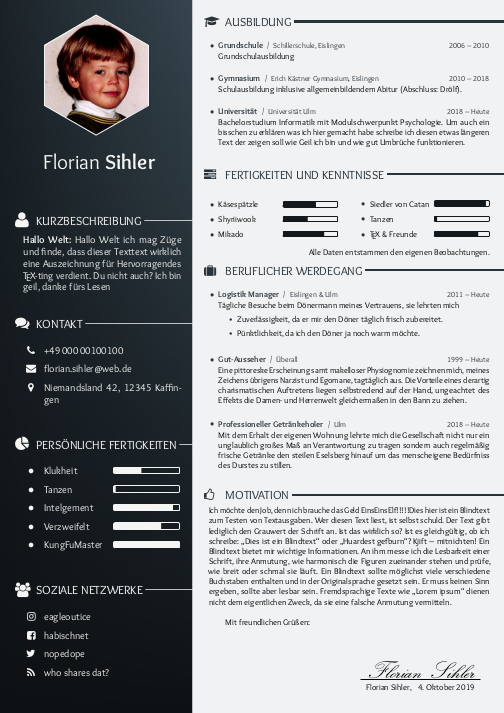
\includegraphics[width=5cm]{Data/Bilder/Application.png}
    \end{minipage}
\end{example}

%
%
%

\presentCommand[2.1.0]{@NeedsFields}[\manArg{csname/tag-list}]
Wird von den Bewerbungs-Designs verwendet um zu überprüfen, ob der Nutzer alle notwenidgen Felder für das jeweilige Thema gesetzt hat. Es obliegt dem Design, ob es Standardwerte für diese Felder liefert. Dieses Paket setzt lediglich das Farbprofil auf \T{Charcoal} (siehe \blankcmd{colorprofile}, gesetzt werden hierbei \typesetList[T]{primary color, secondary color, contrast color, text color, page color} in entsprechend schattierten Farben.)

%
%
%

\presentCommand[2.1.0]{@@applications@Construct@FullName}
Baut aus der Datensammlung den vollen Namen einer Person.

%
%
%

\presentCommand[2.1.0]{@applications@SetNElementsFromCmdListIfTheyExist}[\manArg{max}\manArg{consumer}\manArg{list}]
Setzt bis zu \T{max} Elemente aus \T{list}. Hierbei muss \T{list} die Signatur \T{csname/tag} besitzen. Der \T{consumer} funktioniert analog zu \blankcmd{typesetList}, muss allerdings $4$ Argumente akzeptieren: \blatex{consumer\{current element counter\}\{total element counter\}\{csname\}\{tag\}}. Ein Beispiel findet sich im \T{SimpleLeftBanner}-Design.

%
%
%

\presentCommand[2.1.0]{@applications@SetNElementsFromList}[\manArg{max}\manArg{consumer}\manArg{list}]
Funktioniert analog zu \blankcmd{@applications@SetNElementsFromCmdListIfTheyExist}, allerdings wird eine Liste der Signatur \T{text/tag} erwartet und nicht überprüft ob eine Kontrollsequenz mit diesem Namen existiert.

%
%
%

\presentEnvironment[2.1.0]{application}[\optArg{applicationset}\manArg{design}]
Setzt die Umgebung für eine Bewerbungsseite. Alle folgenden Befehle stehen nur in dieser Umgebung zur Verfügung. Ein Bewerbungsdesign wird mittels \blankcmd{userput} in \blankcmd{lillyPathData} oder unter \blatex[morekeywords={[5]{LILLYxPATHxPRESENTER}}]{:bs:LILLYxPATHxPRESENTER/Showcase/Modules/ApplicationDesigns} gesucht und es besteht aus einer \T{<Name>.tex}-Datei die mit \blankcmd{StartApplication} gesetzt wird und aus einer \T{<Name>.config.tex} die mit dem Start dieser Umgebung geladen wird und so Seitenmaße oder weitere Befehle konfigurieren kann.

%
%
%

\presentCommand[2.1.0]{setname}[\manArg{Name}\cmdlist\anothercmd[2.1.0]{colorprofile}\manArg{color}]
Setzen den Namen beziehungsweise das Farbprofil. Soll beim Namen ein Zweiname angegeben werden so muss dieser extra geklammert werden, als zum Beispiel \T{\blankcmd{setname}\{\{Dieter Jürgen\} Günther\}}.

%
%
%

\presentCommand[2.1.0]{setbrief}[\manArg{init}\manArg{brief}\cmdlist\anothercmd[2.1.0]{setemail}\manArg{email}\cmdlist\anothercmd[2.1.0]{setphone}\manArg{number}\cmdlist\secline\anothercmd[2.1.0]{setmphone}\manArg{number}\cmdlist\anothercmd[2.1.0]{setwebsite}\manArg{url}\cmdlist\anothercmd[2.1.0]{setlocation}\manArg{place}\cmdlist\anothercmd[2.1.0]{setimage}\manArg{path}]
Setzen jeweils die Felder mittels \blankcmd{applicationset}.

%
%
%

\presentCommand[2.1.0]{addskill}[\manArg{name}\manArg{progress}\cmdlist\anothercmd[2.1.0]{addskilltext}\manArg{text}]
Fügt Elemente der Liste an Fertigkeiten zu die in \blankcmd{lilly@applications@skills} gespeichert wird und von den Designs dann enstprechend gesetzt werden kann.

%
%
%

\presentCommand[2.1.0]{StartApplication}
Kann nach dem setzen aller Daten dazu verwendet werden um mit dem setzen des Designs zu beginnen. Auch wenn jedes Design von hier an die Befehle für den Hauptteil selbst setzen kann, so wird grundlegend die folgende Umgebungsstruktur gewünscht: Jeder Abschnitt wird in einem \blankenv{block} gesetzt, in dem dann mit \blankenv{text}, \blankenv{bulletpoints} oder \blankenv{timeline} entsprechende Segmente gesetzt werden können:

%
%
%

\presentCommand[2.1.0]{sign}[\optArg{sign}\optArg[Mit freundlichen\ldots]{Text}]
Sollte außerhalb von \blankenv{block} verwendet werden und erzeugt ein Feld für Unterschriften. Wird \T{sign} übergeben, so wird mit dem entsprechenden Text signiert, sonst wird die Linie freigelassen.

%
%
%

\presentCommand[2.1.0]{block}[\optArg{Symbol}\manArg{Titel}]
Setzt einen neuen Abschnitt im entsprechenden Design. Das Design ist dafür verantwortAppleGreen,Azure,DebianRed,ddpurplelich entsprechende Kurzbefehle zur Verfügung zu stellen. Zu erwarten sind allerdings die folgenden Umgebungen und Befehle.

%
%
%

\presentCommand[2.1.0]{progressbar}[\manArg{progress}]
Setzt eine Fortschrittleiste in den durch \blankcmd{colorprofile} festgelegten Farben.

%
%
%

\presentEnvironment[2.1.0]{bulletpoints}[\optArg{columns}]
Setzt mittels \blankenv{itemize} eine Liste an Punkten, die sich automatisch an die Verschachtelungstiefe anpassen. \blankenv{multicols} wird nur verwendet, wenn eine \T{columns} gesetzt wird.

%
%
%

\presentEnvironment[2.1.0]{timeline}
Primär zur semantischen Trennung. Erlaubt das Verwenden der folgendne Umgebung:

%
%
%

\presentEnvironment[2.1.0]{event}[\manArg{Name}\manArg{Wann}\manArg{Wo}]
Setzt ein Event in einer Zeitleiste.

%
%
%
%
%

\section{Spiele}
\subsection{Kartenspiele}
\hypertarget{LILLYxCARDS}Diese Definitionen werden über die Bibliothek \LILLYxNOTExLibrary{LILLYxCARDS} zur Verfügung gestellt. Sie werden mit \LILLYxBOXxVersion{2.1.0} automatisch mit dem Einbinden von \LILLYxNOTExLibrary{LILLYxPRESENTER} geladen.\medskip\newline

Dieses Paket stellt die Möglichkeit zur Vefügung Spiele mit verschiedenen Spielkarten zu erzeugen, wobei zusätzlich einige Hilfsfunktionen wie \blankcmd{CardFan} angeboten werden:

%
%
%

\presentCommand[2.1.0]{CreateCardGame}[\optArg{card args}\manArg{GameID}\manArg{title}]
Erzeugt ein neues Spiel mit der ID \T{GameID}, diese \emph{muss} eindeutig sein, sonst wird ein bestehndes Spiel überschreiben. Für die Kartenargumente \T{card args} siehe \blankcmd{<GameID>x<ClassID>xNewCard}, der Titel wird nur bei Befehlen wie \blankcmd{ShowGameClasses} angezeigt. Es wird der Befehl \blankcmd{<GameID>xCreateCardClass} erzeugt:

%
%
%

\presentCommand[2.1.0]{<GameID>xCreateCardClass}[\optArg{card args}\manArg{ClassID}\manArg{title}]
Erzeugt eine neue Klasse mit der ID \T{ClassID} für das Spiel \T{<GameID>}, diese \emph{muss} eindeutig sein, sonst wird eine bestehnde Klasse überschreiben. Für die Kartenargumente \T{card args} siehe \blankcmd{<GameID>x<ClassID>xNewCard}, der Titel wird nur bei Befehlen wie \blankcmd{ShowClassCards} angezeigt. Es wird der Befehl \blankcmd{<GameID>x<ClassID>xNewCard} erzeugt:

%
%
%

\presentCommand[2.1.0]{<GameID>x<ClassID>xNewCard}[\optArg{card args}\manArg{CardID}\manArg{title}]
Erzeugt die Karte \T{CardID} in der Klasse \T{<ClasID>} des Spiels \T{<GameID>}. Neben den optionalen \T{card args} die mit der generierung angeführt werden erhält sie auch noch alle Argumente die der Klasse beziehungsweise dem Spiel übergeben wurden. Die Argumente werden durch \T{lillyxCARDSx} persistiert und erlauben die folgenden Konfigurationen:
\begin{center}
    \begin{tabularx}{\linewidth}{^t>{\em}^l^c^p{0.3\linewidth}+}
        \toprule
            \headerrow Bezeichner & \normalfont\bfseries Typ & Standard & Beschreibung\\
        \midrule
            draw & Drawer & default & Routine, die die Karte zeichnen soll \\
            main color & Color & Azure & Hauptfarbe der Karte \\
            back color & Color & MudWhite!25 & Hintergrundfarbe der Karte \\
            border color & Color & Charcoal & Randfarbe der Karte \\
            second color & Color & Azure & Sekundärfarbe der Karte \\
            text style & Tikzargs & white & Formatierungen für (Haupt-) Texte. \\
        \midrule
            extra 1 & Beliebig &  & Register, dessen Bedeutung vom Drawer abhängt. \\
            extra 2 & Beliebig &  & Register, dessen Bedeutung vom Drawer abhängt. \\
            extra 3 & Beliebig &  & Register, dessen Bedeutung vom Drawer abhängt. \\
            extra 4 & Beliebig &  & Register, dessen Bedeutung vom Drawer abhängt. \\
            extra 5 & Beliebig &  & Register, dessen Bedeutung vom Drawer abhängt. \\
            extra 6 & Beliebig &  & Register, dessen Bedeutung vom Drawer abhängt. \\
            extra 7 & Beliebig &  & Register, dessen Bedeutung vom Drawer abhängt. \\
            extra 8 & Beliebig &  & Register, dessen Bedeutung vom Drawer abhängt. \\
            extra 9 & Beliebig &  & Register, dessen Bedeutung vom Drawer abhängt. \\
        \bottomrule
    \end{tabularx}\nskip
\end{center}
Es wird der Befehl \blankcmd{<CardID>} erzeugt.

%
%
%

\presentCommand[2.1.0]{<CardID>}[\optArg{extra Args}]
Ruft die \T{draw}-Routine mit den entsprechendne Konfigurationen für die Karte auf.


\begin{bemerkung}[Das \T{draw} Makro]
    Hier kann jeder beliebige Bezeichner übergeben werden, solange ein Makro der Signatur \blankcmd{@lilly@cards@draw@<Bezeichner>} definiert ist, welches zwei Argumente konsumiert. Für mehr Informationen siehe \blankcmd{@lilly@cards@draw@default}. Dieses Makro wird (auch zum debugging) standardmäig mitgeliefert.
\end{bemerkung}

%
%
%

\presentCommand[2.1.0]{@lilly@cards@draw@default}[\manArg{extra args}\manArg{CardID}]
Übernimmt das Zeichnen einer Informationsübersicht für die Karte. Im Folgenden ein Beispiel:
\begin{defaultlst}[morekeywords={[5]{\\SpielAxCreateCardClass,\\SpielAxKlasseAxNewCard,\\KarteA}}][listing side text,righthand width=2.5cm]{lLatex}
\CreateCardGame[extra 1={Hi}]{SpielA}{Das Spiel A}
\SpielAxCreateCardClass[extra 2={Du}]{KlasseA}{Die Klasse A}
\SpielAxKlasseAxNewCard[extra 3={Na?}]{KarteA}{Die Karte A}
\KarteA
\end{defaultlst}
\CreateCardGame[extra 1={Hi}]{SpielA}{Das Spiel A}
\SpielAxCreateCardClass[extra 2={Du}]{KlasseA}{Die Klasse A}
\SpielAxKlasseAxNewCard[extra 3={Na?}]{KarteA}{Die Karte A}

%
%
%

\presentCommand[2.1.0]{@lilly@cards@get}[\manArg{CardID}\manArg{Key}]
Evaluiert zum persistierten \T{key} der Karte \T{CardID}, leerfelder werden hierbei durch ein \T{@} ersetzt und die Extras mit Buchstaben enummeriert (also zum Beispiel \T{extra@d} anstelle \T{extra 4} und \T{back@color} anstelle \T{back color}).

%
%
%

\presentCommand[2.1.0]{ShowGameClasses}[\manArg{GameID}\cmdlist\anothercmd[2.1.0]{ShowClassCards}\manArg{ClassID}]
Zeigen jeweils eine Vollansicht ihrer jeweils untergeordneten Kategorien (\blankcmd{ShowGameClasses} ruft für jede Klasse zusätzlich \blankcmd{ShowClassCards} auf).

%
%
%
\presentCommand[2.1.0]{CardFan}[\optArg[0]{Risen-List}\manArg{CardID-List}\manArg{max Cards}\cmdlist\secline\anothercmd[2.1.0]{CardBoard}\optArg[0]{Risen-List}\manArg{CardID-List}\manArg{Distance}]
Ordnet die Karten in der jeweiligen Form an. Als optionales Argument können bei $1$ beginnende Indices urchgegeben werden. Diese Karten werden hervorgehoben. Zu der bei \blankcmd{@lilly@cards@draw@default} erstellten Struktur fügen wir hinzu:
\begin{latex}[morekeywords={[5]{\\SpielAxCreateCardClass,\\SpielAxKlasseAxNewCard,\\KarteA,\\KarteB}}]
\SpielAxKlasseAxNewCard[extra 3={Wa?}]{KarteB}{Die Karte B}
\CardFan{KarteA,KarteB,KarteB,KarteA,KarteA}{4}
\CardBoard[2,3]{KarteA,KarteB,KarteB,KarteA}{2em}
\end{latex}
\SpielAxKlasseAxNewCard[extra 3={Wa?}]{KarteB}{Die Karte B}
Ergibt:
\begin{center}
    \CardFan{KarteA,KarteB,KarteB,KarteA,KarteA}{3}\hskip17em\CardBoard[2,3]{KarteA,KarteB,KarteB,KarteA}{2em}\vskip2em
\end{center}
Das Maximum bei \T{max Cards} kann übrigens auch größer sein als die Liste. Die Karten werden dann wahrscheinlich weiter gespreizt gesetzt.

%
%
%
%
%

\subsection{Fantasie-Kartenspiel}
\hypertarget{LILLYxCARDSxFANTASY}Diese Definitionen werden über die Bibliothek \LILLYxNOTExLibrary{LILLYxCARDSxFANTASY} zur Verfügung gestellt. Dieses Paket basiert auf \LILLYxNOTExLibrary{LILLYxCARDS} (mit dem es ebenfalls geladen wird) und definiert neben dem neuen \T{draw} namens \say{fantasy} die folgende Umgebung zur einfachen Generierung von Karten (genau genommen stellt diese Umgebung nur Umbenennungen für \blankcmd{<CardID>} zur Verfügung.) Der Drawer verwendet die Extras wie folgt:
\begin{multicols}{3}
    \begin{enumerate}
        \item Bildpfad
        \item Kartenkosten
        \item Farbe des Kostenfelds
        \item Kartensymbol
        \item Kartenfarbe
        \item Zitat
        \item Effekt
    \end{enumerate}
\end{multicols}

%
%
%

\presentEnvironment[2.1.0]{NewFantasyCard}[\optArg{card args}\manArg{GameID}\manArg{ClassID}\manArg{CardID}]
In dieser Umgebung stehen die folgende Befehle zur Verfügung, die die entsprechenden Felder setzen: \typesetList[blankcmdidx]{settitle,setimage,setprice,setpricecolor,setclasssymbol,setclasstext,setquote,seteffects,setcolor,setcardcolor,settextstyle}.

\begin{bemerkung}[Einen Helden erschaffen]
    Im Folgenden gilt es mich, den Autor als Magier-Karte zu etablieren. Wir beginnen mit der Erzeugung es Spiels:
    \begin{latex}
\CreateCardGame[draw=fantasy, extra 3={ChromeYellow}]{Fantasy}%
        {Ein Fantasy-CardGame}
    \end{latex}\CreateCardGame[draw=fantasy, extra 3={ChromeYellow}]{Fantasy}{Ein Fantasy-CardGame}%
    Wir setzen also die Farbe des Preisfeldes für alle Karten in diesem Spiel auf \T{ChromeYellow}, wuhuu \Smiley. Nun erstellen wir die Magier-Klasse wobei ich auf das \T{fontawesome}-Symbol \T{faMagic} zurückgreife:
    \begin{latex}[firstnumber=last,morekeywords={[5]{\\FantasyxCreateCardClass,\\magicLogo}}]
\def!**!\magicLogo{\large!**!\faMagic}
\FantasyxCreateCardClass[extra 4={\noexpand!**!\magicLogo}, %
        extra 5={Magier}, main color={Purple}]{Mages}{Die Magier Klasse}
    \end{latex}\FantasyxCreateCardClass[extra 4={\noexpand\large\noexpand\faMagic}, extra 5={Magier}, main color={Purple}]{Mages}{Die Magier Klasse}%
    Nun erstellen wir die Karte mittels \blankenv{NewFantasyCard}:
    \begin{latex}[firstnumber=last,morekeywords={[5]{\\FantasyxCreateCardClass}}]
\begin{NewFantasyCard}{Fantasy}{Mages}{Flo}
    \settitle{Florian der Zauberer}
    \setimage{Data/me.jpg}
    \setprice{42}
    \setquote{\say{Ich werde dich mit Blicken vernichten! Schauangriiiiiiiiiff!!!}}
    \seteffects{\medskip%
        \begin{itemize}[leftmargin=14pt]\closeritems
            \item Sieht verdammt gut aus.
            \item Schrecken aller Magier.
            \item Beherrscht: Klingentanz. Ja! Als Magier!
        \end{itemize}\medskip
        {\scriptsize Super EPIC POWER}
    }
\end{NewFantasyCard}
    \end{latex}
    \begin{NewFantasyCard}{Fantasy}{Mages}{Flo}
        \settitle{Florian der Zauberer}
        \setimage{Data/me.jpg}
        \setprice{42}
        \setquote{\say{Ich werde dich mit Blicken vernichten! Schauangriiiiiiiiiff!!!}}
        \seteffects{\medskip%
            \begin{itemize}[leftmargin=14pt]\closeritems
                \item Sieht verdammt gut aus.
                \item Schrecken aller Magier.
                \item Beherrscht: Klingentanz. Ja! Als Magier!
            \end{itemize}\medskip
            {\scriptsize Super EPIC POWER}
        }
    \end{NewFantasyCard}
    Natürlich würde man sich selbst Kurzbfehle und Stile für die Effekte definieren, die einfach übergeben werden können. Hier übrigens noch das Ergebnis, auf das wir alle gewartet haben: \iflillycompact\else\begin{center}
        \Flo
    \end{center}\fi
\end{bemerkung}